\documentclass[12pt,a4paper,fleqn]{article}
\usepackage{rmpackages}																% usual packages
\usepackage{rmtemplate}																% graphic charter
\usepackage{rmexocptce}																% for DS with cptce eval

%\cfoot{} 													% if no page number is needed
%\renewcommand\arraystretch{1.5}		% stretch table line height

\begin{document}

\begin{header}
\Large
De quelle couleur sont les étoiles les plus chaudes ?
\end{header}

\begin{multicols}{2}
\begin{center}
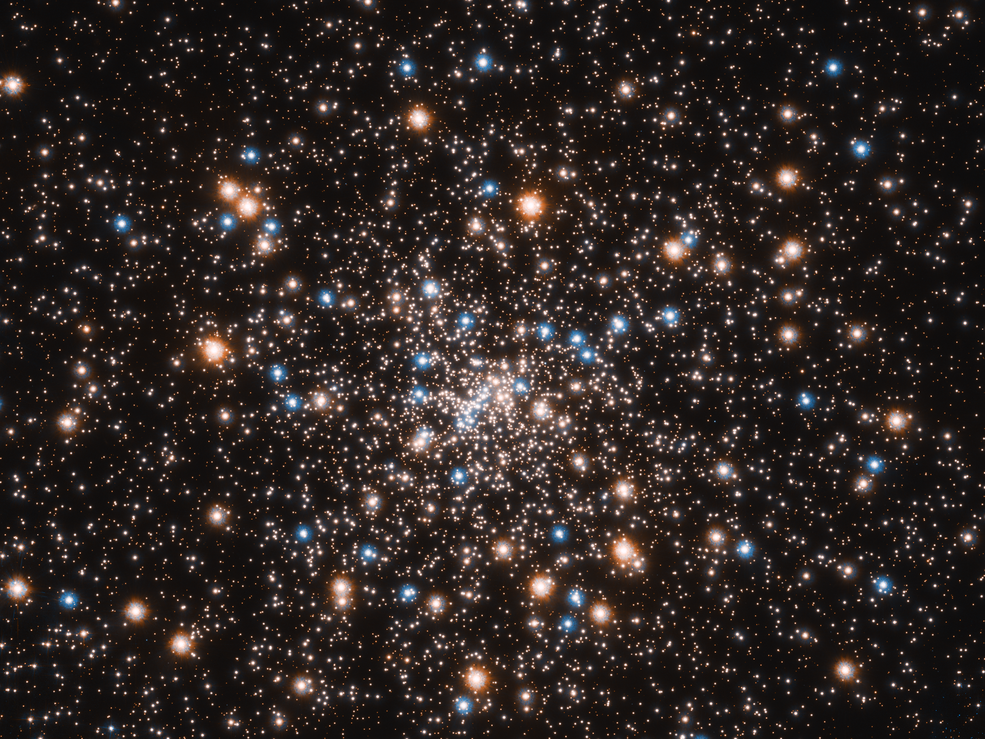
\includegraphics[trim=0 130 0 130, clip, width=\linewidth]{images/hubble_globular_cluster.png}
\end{center}

Comme le filament d'une ampoule ou une barre de métal chauffée à blanc, les étoiles sont des corps chauds (très chauds) qui émettent de la lumière.

On veut établir le lien entre la température d'une étoile et sa couleur, ce qui permet d'étudier précisément certaines de leurs caractéristiques même si elles sont situées très loin de nous.
\end{multicols}

\begin{enumerate}
\item \anarai{}
\label{quest:hyp}

Notez votre hypothèse justifiée.
\end{enumerate}

\begin{center}
\begin{tikzpicture}
\draw [color=white] (0,.5) -- ++ (.99\linewidth, 0);
\foreach \i in {0,1} {
  \draw [color=gray_c] (0,-.9*\i) -- ++ (.99\linewidth, 0);
}
\end{tikzpicture}
\end{center}

On ne peut pas mesurer directement la température d'une étoile.
On va donc tout d'abord utiliser une lampe à incandescence dont on peut modifier la température du filament.

\begin{enumerate}[resume]
\item \rea{}

Faire un schéma de l'expérience à réaliser pour obtenir le spectre du rayonnement de la lampe.%
\thumbsup{}

\vspace{150pt}
\end{enumerate}

\begin{appel}
\rea{}
\end{appel}

Pour plusieurs températures différentes, on observe les spectres ci-dessous.
\vspace{120pt}

\begin{enumerate}[resume]
\item \app{} \anarai{}

Comment évolue la composition du spectre en fonction de la température ? \thumbsup{}

\end{enumerate}

\begin{center}
\begin{tikzpicture}
\draw [color=white] (0,.5) -- ++ (.99\linewidth, 0);
\foreach \i in {0,1,...,4} {
  \draw [color=gray_c] (0,-.9*\i) -- ++ (.99\linewidth, 0);
}
\end{tikzpicture}
\end{center}

\section*{Température et couleur des étoiles}

Les images ci-dessous montrent la couleur et les spectres de quelques étoiles \og proches \fg{}.

\begin{center}
\newcommand{\localheight}{75 pt}
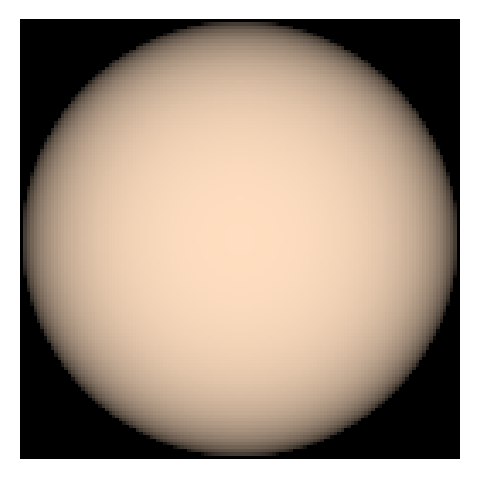
\includegraphics[height=\localheight]{images/star_tau_ceti.png}

\includegraphics[height=\localheight]{images/spectrum_star_tau_ceti.png}

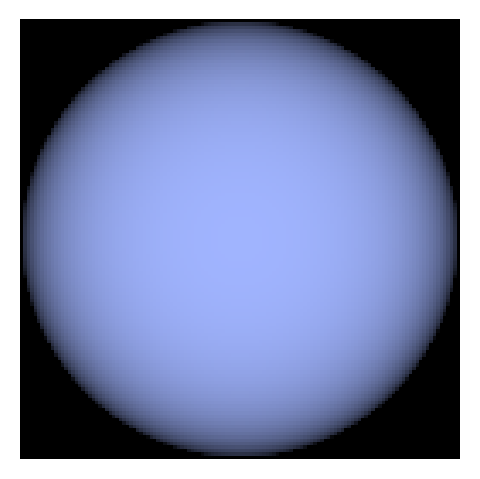
\includegraphics[height=\localheight]{images/star_rigel.png}

\includegraphics[height=\localheight]{images/spectrum_star_rigel.png}

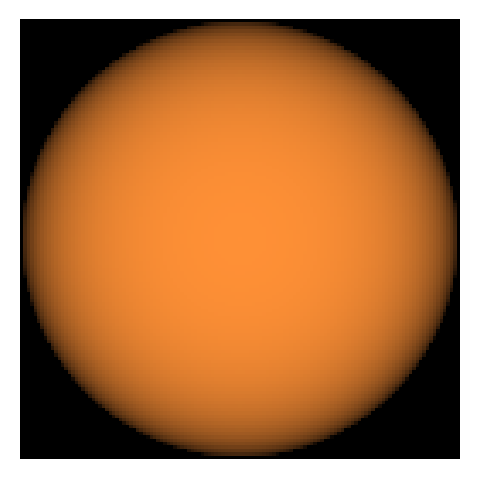
\includegraphics[height=\localheight]{images/star_proxima_centauri.png}

\includegraphics[height=\localheight]{images/spectrum_star_proxima_centauri.png}
\end{center}

\begin{enumerate}[resume]
\item \anarai{}

Classer ces étoiles de la plus froide à la plus chaude. \thumbsup{}

\end{enumerate}

\begin{center}
\begin{tikzpicture}
\draw [color=white] (0,.5) -- ++ (.99\linewidth, 0);
\draw [color=gray_c] (0,0) -- ++ (.99\linewidth, 0);
\end{tikzpicture}
\end{center}

\begin{enumerate}[resume]
\item \val{}

Ces observations confirment-elles votre hypothèse de la question~\ref{quest:hyp} ?
\end{enumerate}

\begin{center}
\begin{tikzpicture}
\draw [color=white] (0,.5) -- ++ (.99\linewidth, 0);
\foreach \i in {0,1} {
  \draw [color=gray_c] (0,-.9*\i) -- ++ (.99\linewidth, 0);
}
\end{tikzpicture}
\end{center}
\vfill

\begin{appel}
\val{}
\end{appel}

\end{document}